\label{developmentIntroduction}
A web application was developed and a CNN was trained in order to fulfill the goals of this thesis. The architecture of the application is portrayed in Figure \ref{ApplicationArchitecture}. 

\begin{figure}[ht!]
  \centering
  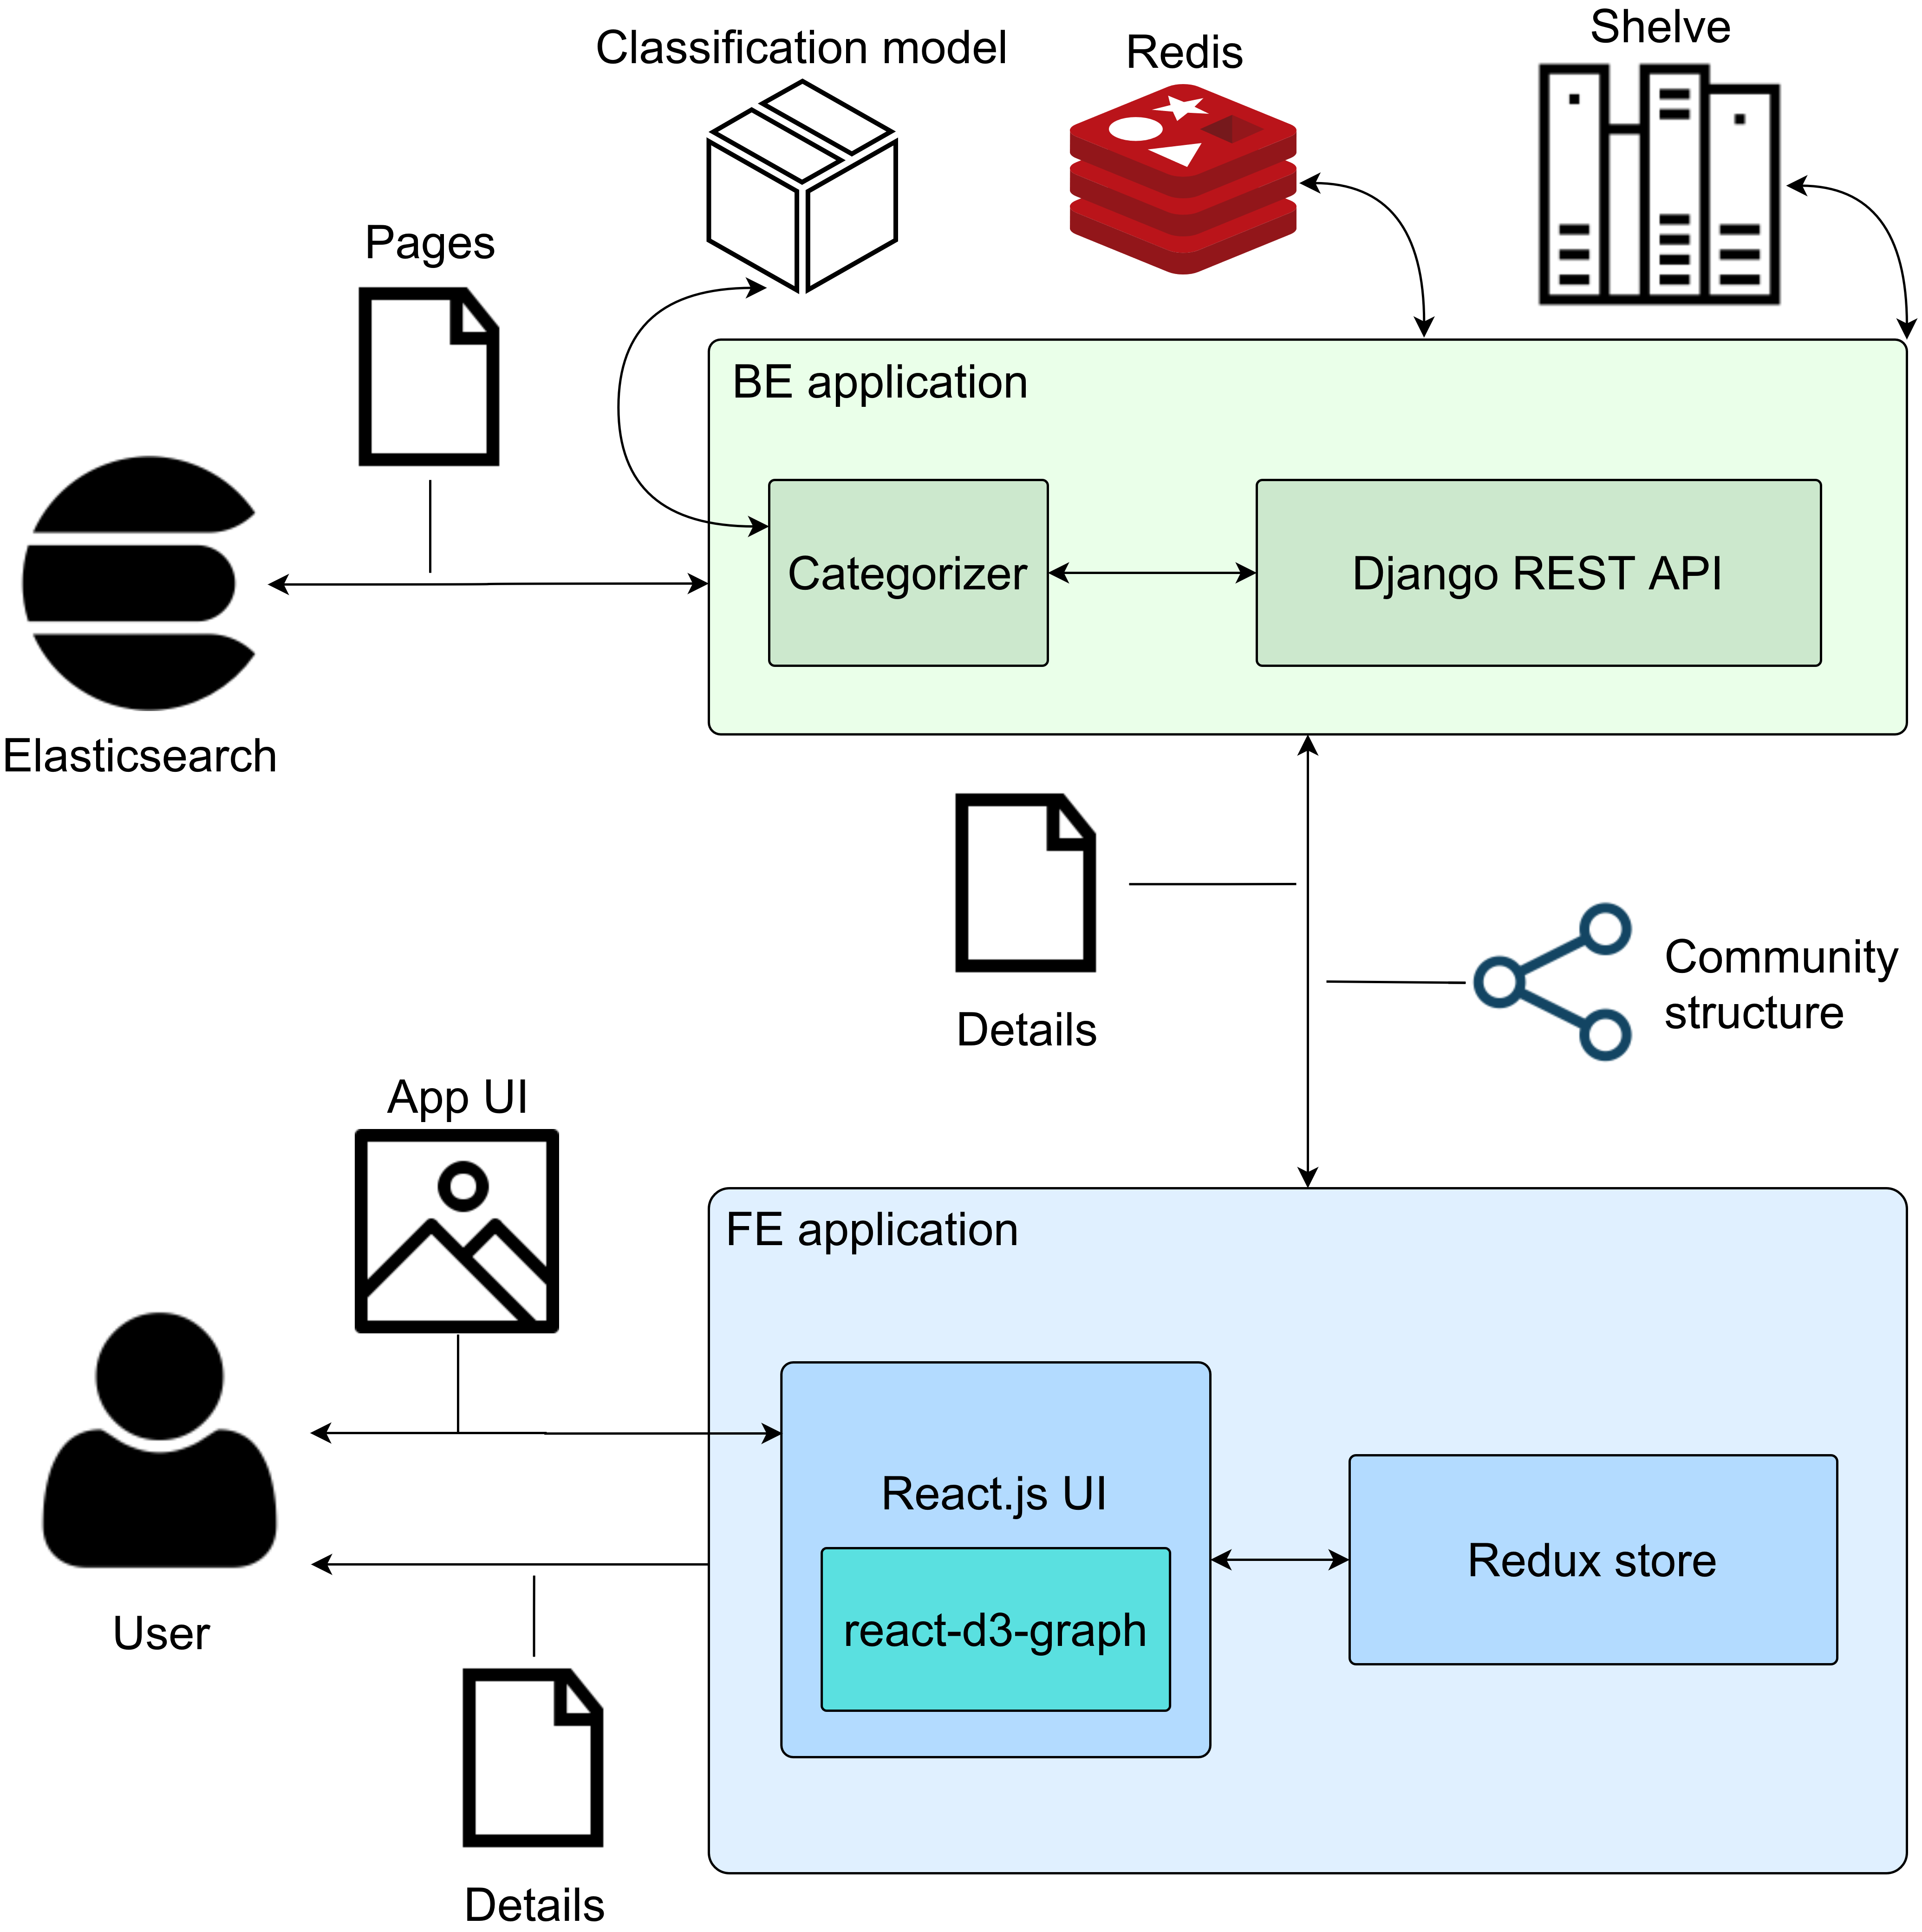
\includegraphics[width = \textwidth]{Images/ApplicationArchitecture.png}
  \caption{The visualization of the architecture of the web application.}
  \label{ApplicationArchitecture}
\end{figure}

One task of the application was to classify the scraped pages into categories. This was to be done depending on the content of the pages. The application performs the classification via the model created by the CNN. CNNs and ANNs are described in Section \ref{artificialNeuralNetworks}. 

Another task was to provide a way to observe the structure of the pages, links between them, and their categories. This was achieved by detecting communities of a graph. Communities and how to detect them are described in Chapter \ref{clustering}. 

One of the partner requirements was for the application to function on a UNIX system. Another requirement was a user friendly user interface (UI). Also, the option for the retrieval of all the available information about the pages was expected. 

This chapter first describes the implementation of the model for the classification of the pages. Afterwards the implementation of the clustering is introduced. Then the design and implementation of the application which is composed of a back-end application (BE) with a representational state transfer (REST) application program interface (API) and a front-end (FE) web application is detailed. 

\section{Classification} \label{ClassificationDevelopment}
To categorize the pages depending on their content a CNN needed to be created. The number and the structure of the available data are detailed in Section \ref{dataSet}. A project called \texttt{Categorization} was built. For the training of a CNN a suitable training and testing data set needed to be prepared. The desired output of the CNN was a model able to categorize the pages with a reasonable accuracy. 

This chapter describes the steps taken in order to achieve the listed goals along with the technologies used.

\subsection{Technology overview} \label{ClassificationTechonologyOverview}
The project was written in \textit{Python}. \textit{Python} is a widely used interpreted programming language known for readability and portability \cite{aboutPython}. It is open-source and is considered to have an extensive documentation and community available. \textit{Python} is popular in the science community because it is easy to learn and has simple syntax. There is therefore a considerable amount of useful libraries for research purposes such as \textit{Keras}, described later in this subsection, or \textit{igraph}, introduced in Subsection \ref{ClusteringTechonologyOverview}.  

The learning approach used in this thesis was SLr introduced in Subsection \ref{supervisedLearning}. A sample data set with assigned categories was therefore needed. To view and edit a data set with thousands of rows the software \textit{EmEditor} \cite{emeditor} was leveraged. 

\textit{EmEditor} is a paid text editor with a free trial period. The advantage of this editor is its support of large files. Supported file formats include comma-separated values (CSV) files. 

For the modification of the content of the pages we utilized the library \textit{Natural Language Toolkit} (NLTK) \cite{nltk}. \textit{NLTK} is a \textit{Python} library used for operating on human language data. \textit{NLTK} provides functionality such as tokenization, or stemming. The library supports several languages including English. This library comes with detailed documentation. The classification of this thesis supports only English.

For the management of large matrices and vectors we used the library \textit{NumPy} \cite{numpy}. \textit{NumPy} is a \textit{Python} library used for scientific computing. The functionality includes for example the formation of n-dimensional array objects, the random shuffling of rows of such an object, and random number capabilities. 

To manipulate the data set efficiently the \textit{pandas} library \cite{pandas} was adopted. \textit{Pandas} is an open-source library used for the manipulation of data frame\footnote{A data frame is a two-dimensional structure resembling a common table. Data stored in columns contains values designated to the same purpose. } objects. It is possible to slice through, add data to, or remove data from data frames. Also, data frames may be merged or reshaped. Supported file formats include CSV and excel spreadsheet (XLS) files.

The CNN itself was created with the library \textit{Keras} \cite{keras}. \textit{Keras} is a library for the implementation of ML in \textit{Python}. ML is depicted in Section \ref{machineLearning}. \textit{Keras} supports the tokenization of text and the tools needed to build and train a CNN. The output model of the CNN can be used for the task it was trained for.

\subsection{Learning data set} \label{LearningDatasetImplementation}
A labeled data set for learning was necessary. We therefore built a learning data set composed of a subset of the scraped pages. The pages were retrieved from the database with equivalent fetching functionality as is described in Subsection \ref{APIImplementation}. This functionality is located in the folder \texttt{helpers}. Only one page with content of each domain from the Tor network was stored. 4,088 pages were obtained this way. These pages were with content exported into a CSV file and labeled manually. 

13 categories were identified. We will call this learning data set \textit{first samples} in a later chapter. The problem of this data set was some categories contained less than 100 pages. The training result for those categories were not satisfying. Detailed training results performed on various training data sets are shown in Section \ref{classificationEvaluation}. 

By the merging of categories with less than 100 pages into bigger categories we achieved better training results. One category, \textit{Gambling}, could not be merged with other categories as it was not related enough to any other category. We therefore enhanced \textit{Gambling} with more pages from the database. This was possible because we found a domain with more than 200 pages with different content all associated to gambling. This data set contained 4.298 pages and 10 categories. We will further call this learning set \textit{enhanced samples}. However, a moral issue related to the naming conventions of the categories arose with this data set. 

The final data set was created by further merging and renaming the categories. 9 categories were identified. We will call this data set \textit{final samples}. The 9 categories detected are detailed as follows:
 \label{classificationCategories}
\begin {description}
	\item[Finance and Fraud] contained 665 pages. It included content about fake or stolen credit, debit, and gift cards and bank accounts. Also crypto currency, counterfeit money, and money laundering was mentioned. Suspicious and illegal investment opportunities were offered as well.
	\item[Gambling] contained 231 pages. Content involving casinos, bets, and other form of gambling constituted this category.
	\item[Hosting and Programming and Hacking] contained 411 pages. Content assigned with this category involved technical blogs and hosting servers. Hacking tutorials and services were also offered.
	\item[Illegal services and goods] contained 139 pages. Provided services involved the hiring of hitmen\footnote{A hitman is person hired to kill another person or people.} and fake identity services. Offered goods included drugs and guns.
	\item[Online Marketplace] contained 143 pages. Content labeled with this category consisted of mentioning products of other categories along with electronics, clothing and accessories. All of these goods were offered at once on one page.
	\item[Other] contained 806 pages. Pages in this category were not possible to categorize. The content was either not English, too incoherent, short, or vague. 
	\item[Sexual Content] contained 1,196 pages. Content in this category was of a sexual nature including sexual stories and the mentioning of images or videos.
	\item[Social] contained 136 pages. This content included blogs, chat rooms, and information channels. Also censored content was found, such as the Bible or confidential information. Other content present was written works of art and mentions about paintings and music. 
\end{description}

\subsection{Implementation} \label{ClassificationImplementation}
The preprocessing of the learning data and the training of the CNN takes place in the file \texttt{keras\_classification\_model.ipynb}. 

The learning data are loaded as a data frame. The data preprocessing is performed on the content of the pages. Non-English rows, also called documents, are removed. Documents below a 20\%  threshold of English content are discarded. The threshold was chosen after discussions with the supervisor. The removal of non-English documents is described in detail in Appendix \ref{dixRemoveNonEnglish} 

Next, the labels are to be pre-processed as CNNs require labels to be represented by integers. For that, the labels are retrieved from the data frame by removing duplicates from the category column. Then a dictionary\footnote{A python dictionary is a hash table with keys and values.} with the category name as key and the index\footnote{An index in context of this chapter is an integer value corresponding to the position of an entry. It starts from 0.} as value is created. The indexes are used as category aliases. This dictionary functions as a category--index lookup table.

Afterwards, two empty lists are initialized, \texttt{texts} and \texttt{labels}. For each row of the data frame the content is appended to list \texttt{texts}, the category is converted to the matching alias and appended to the list \texttt{labels}. The text is associated with the analogous label by making use of the indexes in the individual lists lists.  This is explained on an example. The row on position $i$ contains content $T_i$ and the corresponding category $C_i$. Content $T_i$ is appended to \texttt{texts} and is on the $i$th position. The alias for category $C_i$ is $C^a_i$. Now $C^a_i$ is appended to \texttt{labels} and is also on the $i$th position.

Next an internal vocabulary is initialized from all words from \texttt{texts}. The list \texttt{texts} corresponds to a matrix. The matrix is stored in a list of matrices called \texttt{data}. The list \texttt{data} is split into a training and testing set. One fifth of \texttt{data}, meaning 864 entries, is randomly chosen to be the test set. The rest are the training data. 

Each category alias in \texttt{labels} is assigned an index $i$. Each entry of the list is replaced by a one hot vector (OHV)\footnote{A zero vector with one value being 1.} . The value 1 is on the $i$th position of the OHV. The length of the OHV coincides to the number of categories. The list \texttt{labels} becomes a matrix after this modification, meaning a list of vectors. It then is also separated into training and testing data in accordance with the \texttt{data} division.

The next step is the configuration of embeddings. Embeddings are outlined in Subsection \ref{embeddingLayers}. An open source embedding matrix is available on the Stanford university web site \cite{embeddings}. However, using that matrix changed the learning results only marginally as opposed to training the EmbL on our data. One of the reasons might be the vocabulary and the content syntax of the dark web being different from the vocabulary used in the pre-trained embeddings file. We therefore decided not to use the Stanford embeddings. An example of an embedding vector is enclosed in the Appendix \ref{dix_embeddingVector}.

The last step before the training itself is to create the shape of the CNN. The \textit{Keras} documentation offers a sample of a CNN structure meant for text classification \cite{kerasCNNStructure}. We adopted the sampled structure. Figure \ref{structureOfCNN} depicts the structure composition. 

The EmbL receives information about the vocabulary size, the number of words on each page, and the length of the output vectors. The vocabulary is limited to 20,000 most frequently occurring words. The number of words in the content of each page is limited to 1,000. The EmbL therefore expects an input of vectors with length 1,000. The output of this layer are embedding vectors with length of 100. 

The second layer is a 1D ConvL with 128 neurons and a kernel with the dimensions 5x1. The AcF of this layer is ReLU described in Subsection \ref{activationFunction}. Next a PoolL with filter dimensions of 5x1 is prepared. The method used in the pooling layer is max-pooling. The next layer is a 1D ConvL followed by a PoolLr and another 1D ConvL all equivalent to the first layers of the corresponding types. The seventh layer is a PoolL also using max-pooling but with the filter dimensions equal to the input dimensions. Then a DnsL with 128 neurons and ReLU as its AcF follows. The last layer is another DnsL with the AcF softmax. The number of neurons in this layer is the number of categories. In our case 9.

Afterwards a \textit{Keras} model is fed the CNN structure and compiled. The configured LsF of the model is CCross. The desired metrics to be evaluated is the accuracy of the results. The optimizer used is RMSprop. The model is then trained on the training and testing data. The number of epochs is set to 20 and batch\_size is 128.

After the training finished the model was exported. It then was used in the BE for the categorization of the pages.




\section{Clustering}\label{ClusteringDevelopment}
The structure of the pages was to be visualized in the form of a web graph. The amount of the pages described in Section \ref{dataSet} needed to be divided into communities in order to view the structure without the loss of information. For this purpose both the LA and the LeA were used, separately. These algorithms are characterized in Section \ref{louvainAlgorithm} and Section \ref{leidenAlgorithm} respectively. 

\subsection{Technology overview} \label{ClusteringTechonologyOverview}
In the beginning we used the library \textit{NetworkX} \cite{networkX} for the graph creation. \textit{NetworkX} is a \textit{Python} library for the managing of complex networks. The advantage of this library is convenient documentation. Also, the graphs of \textit{NetworkX} cover many characteristics such as undirected and directed, or weighted edges. It is possible to filter isolates from the graph. Another advantage is the availability of standard graph algorithms, including the LA. However, the built in LA implementation was too slow for the size of our data set. It didn't succeed to divide about 40,000 pages within 30 minutes. We therefore decided to use a different implementation. The \textit{cylouvain} library \cite{cylouvain} was introduced. 

\textit{Cylouvain} is a faster implementation of the LA. The division of 90,275 pages into communities took about 15 seconds. The problem we faced with this implementation was the occasional occurrence of disconnected sub-communities of communities. 

Our new priority was therefore to adopt an implementation of the LeA. The \textit{leidenalg} \cite{leidenalg} library was introduced. \textit{Leidenalg} is a \textit{C++} implementation of the LeA exposed to \textit{Python}. This implementation takes about 6 seconds to partition the 90,275 pages into communities. Moreover, there are no disconnected sub-communities of communities. \textit{Leidenalg} is built on the \textit{python-igraph} (igraph) library. 

\textit{Igraph} is another library for the managing of complex networks. The advantage of this library the availability of the before mentioned implementation of the LeA.

We decided to keep the LA implementation despite the drawbacks for comparison purposes. The two utilized implementations are compared in Section \ref{clusteringEvaluation}.

\subsection{Implementation} \label{ClusteringImplementation}
The clustering is implemented in the BE. The BE is further described in the next Section \ref{APIDevelopment}. We describe the clustering in this subsection. 

The clustering itself (cluster cycle) is executed in the method \\ \texttt{get\_groups\_without\_links\_and\_isolates} in the \texttt{graph\_helpers.py} file. The entry parameter are either scraped pages or communities. Both will act as nodes. The implementations of the clustering algorithms mentioned in the previous Subsection \ref{ClusteringTechonologyOverview} require the nodes to be in a compatible Graph format. 

First, the pages need to be converted into integer aliases. The aliases will constitute the vertices of the graph. The page links also need to be in the form of integer aliases. These link aliases will compose the edges of the graph.

 For the graph initialization one of the libraries \textit{igraph} or \textit{NetworkX} is utilized. The decision is made based on a boolean flag whether to use the LA. The graph is now filled with the edges and the vertices. Next, isolates are filtered out and deleted from the graph vertices. 

Afterwards the communities are detected, the result is a partition. The partition is a dictionary with the node aliases as keys and the communities assigned to the nodes as values. Lastly the aliases in the dictionary are converted back to the original node \textit{ids}\footnote{\textit{Ids} in case of pages are urls. \textit{Ids} in case of communities are specific strings, e.g.~\textit{2.14.0}.}. The method returns the partitioned node ids, and the isolates if any were present. 

\begin{figure}[ht!]
  \centering
  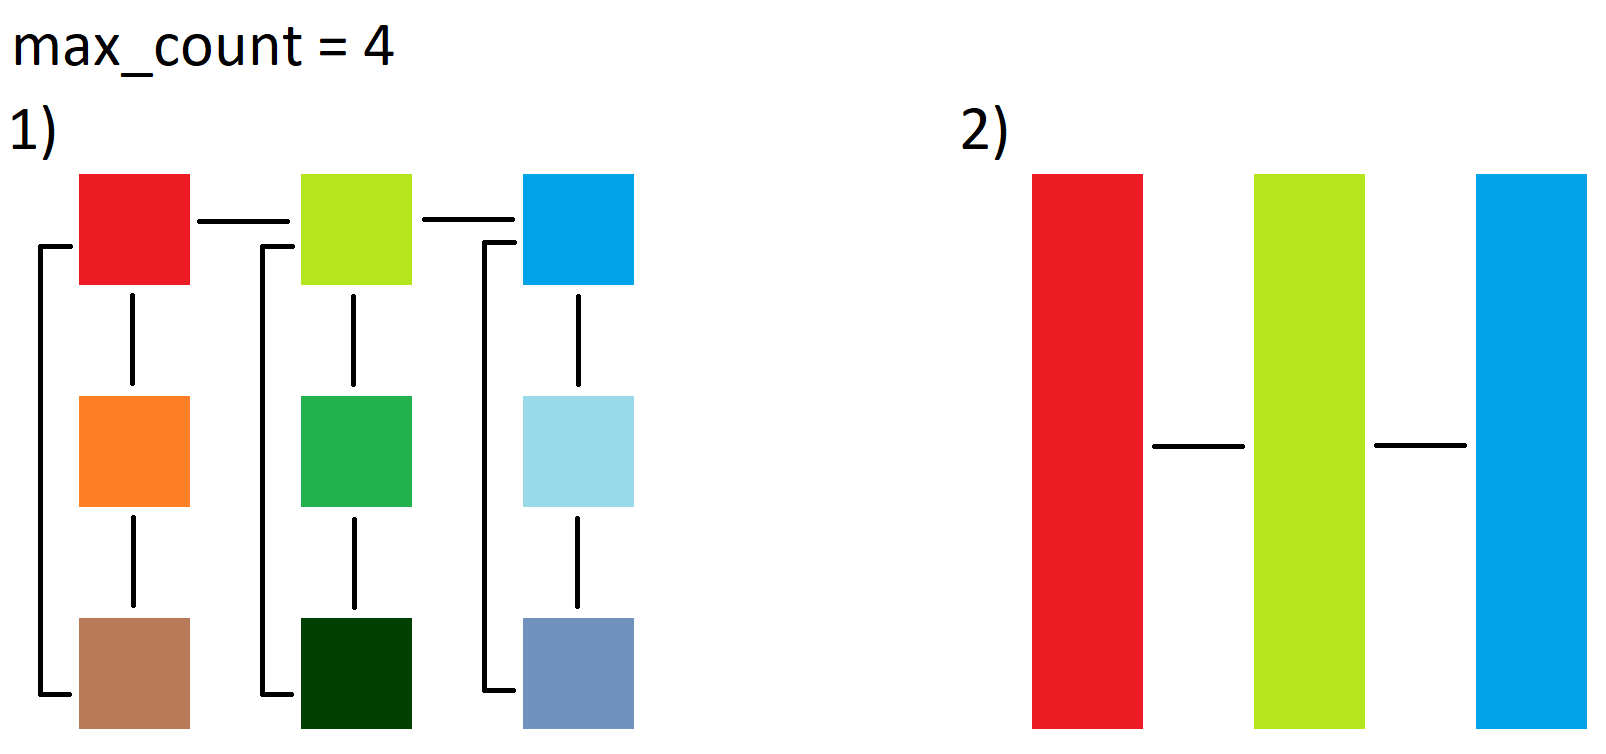
\includegraphics[width=\textwidth]{Images/clusteringCyclesExample.png}
  \caption{An example of multiple cluster cycles. Max count is four. The image on the left represents a hypothetical output of the first cluster cycle. It contains 9 squares each of a different colour with undirectional links between them. Each square depicts a community. The number of the communities is bigger than max\_count. Therefore the cluster cycle is repeated with the 9 communities as the nodes to be clustered. The second cluster cycle detects three communities portrayed as rectangles in the right image. This number satisfies the max count condition and the cluster cycle is not repeated.}
  \label{clusteringCyclesExample}
\end{figure} 

The clustering cycle is repeated on communities until the number of the detected communities is not greater than the desired maximum number (max count). This is demonstrated in Figure \ref{clusteringCyclesExample}. Another reason to end the repetition is if the number of detected communities cannot be reduced any further. Max count in this thesis is 30. This number represents the quantity of communities which is still displayable without major cluttering.




\section{API}\label{APIDevelopment}
The scraped pages of the dark-web were being stored in \textit{ElasticSearch}. We created a BE in order to perform various operations on the data-set before sending it to the FE. Such operations involve resource intensive processing of large volumes of data, and caching. We decided to initialize the BE utilizing \textit{Python}. The reason behind this decision was the requirement for the application to function on a UNIX system. Other reasons are described in Subsection~\ref{ClassificationTechonologyOverview}. 

The required API tasks were the categorization of the nodes along with their division into communities. Communities were represented by either nodes of the same category or by communities. The BE was also demanded to return details for specific pages or groups if requested.


\subsection{Technology overview}
\label{technologyOverview}
The BE was written in \textit{Python\textit} and contained the API. As we wanted our API to follow the REST architecture we decided to make use of the \textit{Django} framework \cite{meetDjango}. \textit{Django} is responsible for tasks such as running the server or managing web requests. Another advantage of \textit{Django} is its \textit{Django REST framework} (DRF). \textit{DRF} offers a convenient way for creating restful endpoints and responses \cite{djangoRest}. Both frameworks are open-source with helpful documentation and community. 

We had to solve performance issues. It took approximately 30 minutes to retrieve and categorize about 220,314 pages from the database and circa 6 seconds to divide such a response into communities. We considered this wait time to be too long. We therefore decided to cache the data of the first response. For that purpose \textit{Redis} \cite{redis} was used. 

\textit{Redis} is an open-source solution which we used as a key-value store. It supports basic data structures\footnote{Simple structures, e.g. strings, numbers or sets.} as values, but not custom objects. Since the API uses custom objects for \textit{communities}, \textit{pages}, or \textit{links}, an object serializer was leveraged along with \textit{Redis}. We decided not to write our own but to utilize the \textit{Python} \textit{pickle} module\footnote{A module used for converting \textit{Python} objects to streams of bytes and vice versa.} \cite{pickle} (pickle). The reason behind this decision was the simplicity of \textit{pickle}. \textit{Pickle} also fulfilled all our needs for serializing. Specifically the serialization or deserialization of data in the form of the previously mentioned models for \textit{Redis} to store in an acceptable time. 

\textit{Pickle} took about 6 seconds to serialize 220,314 pages. The deserialization of the same number of pages took about 7 seconds. However, the combination of \textit{pickle} and \textit{Redis} was not stable enough for the storing of sizable objects. \textit{Redis} and \textit{pickle} were therefore used only for the caching of pages without page content. However, the acquisition of page content was one of the tasks needed of this thesis. As the content was a sizable object we decided to utilize the \textit{Python} module \textit{shelve} \cite{shelve}. \textit{Shelve} manages \textit{shelfs}. A \textit{shelf} file is a persistent \textit{Python} dictionary. The advantages of using \textit{shelve} are the possibility of storing large objects and no need for serialization of keys or values. \textit{Shelve} took approximately 61 seconds to retrieve 220,314 pages with content. 



\subsection{Implementation} \label{APIImplementation}
This API handles the following four use-cases. 
\begin{enumerate}
    \item The acquisition of all, or specific pages divided into communities depending solely on links between the pages. Or the acquisition of a specific page.
    \item  The community detection of all, or specific pages based on categories. This means on the highest level the pages are divided into groups solely by page category. On lower levels the pages are divided into communities depending on the links between the pages.
    \item The obtaining of further details of a specified page.
    \item The retrieval of group details\footnote{Page details of all pages belonging into a specified community.}. 
\end{enumerate} 
It is not possible to obtain sub-communities of communities detected on the specific pages.

The BE is implemented in the project \texttt{Dark-web-categorization-BE}. The project was initialized in the \texttt{category} folder. The \texttt{settings.py} and \texttt{wsgi.py} files were included in the \textit{Django} boilerplate. The file \texttt{urls.py} contains the endpoints for the whole project. The urls relevant to this thesis are from the \texttt{api} module and imported into this file.
The \texttt{api} module is situated in the \texttt{api} folder. The implementation relevant for this thesis is situated here. We now detail the most important files and modules. 
\begin{description}
    \item[\texttt{view\_sets}] contains ViewSets\footnote{A ViewSet is a class which provides responses according to the received parameters. The request methods \textit{GET} and \textit{POST} are supported.} of the API.
    \item [\texttt{urls.py}] registers routes with corresponding \textit{ViewSets} to a \textit{Django} \textit{router}\footnote{An object which assigns ViewSets to the corresponding endpoints.}.
    \item[\texttt{apps.py}] holds the boilerplate configuration file for the API.
    \item[\texttt{classification}] module contains the categorization functionality.
        \begin{itemize}            
            \item[--] \textbf{\texttt{labels.py}} lists the available categories with the corresponding indexes. 
            \item[--] \textbf{\texttt{categorizer.py}} encompasses the class \texttt{Categorizer} used for the categorization in the BE. Implementation details are included in Appendix \ref{dixApClassification}.
        \end{itemize} 
    \item[\texttt{models.py}] accommodates the \textit{Django} models\footnote{A class containing the fields and behaviour of data.}. The models and the relationships between the models are visualized in Appendix \ref{dixModels}. 
    \item[\texttt{serializers.py}] contains serializers\footnote{A serializer transforms \textit{Django} models into different formats, e.g. JSON.}. Each model used in the client-server communication has a matching serializer assigned. An example of handling a response is detailed in Appendix \ref{dixAPIResponse}.
    \item[\texttt{utils}] module encompasses various helper methods. These methods are leveraged for example for the partitioning of the graph, caching, or page detail gathering.
    \item[\texttt{repositories.py}] holds the methods which handle the fetching from the database. More information about the methods in this file are included in Appendix \ref{dixRepositories}
    \item[\texttt{tests}] module contains unit tests
\end{description} 





\section{Front-end}
In order to display the data acquired from the BE in a reasonable way a FE was created. The goal of the FE was to visualize the scraped pages as a web graph. The pages or communities, and links from the BE were to depict nodes, and links of the graph respectively. The categories of the nodes needed to be readable in the graph. Additional information about the nodes needed to be displayed or retrievable on demand.

\subsection{User interface} \label{FEUI}
\begin{figure}[ht]
  \centering
  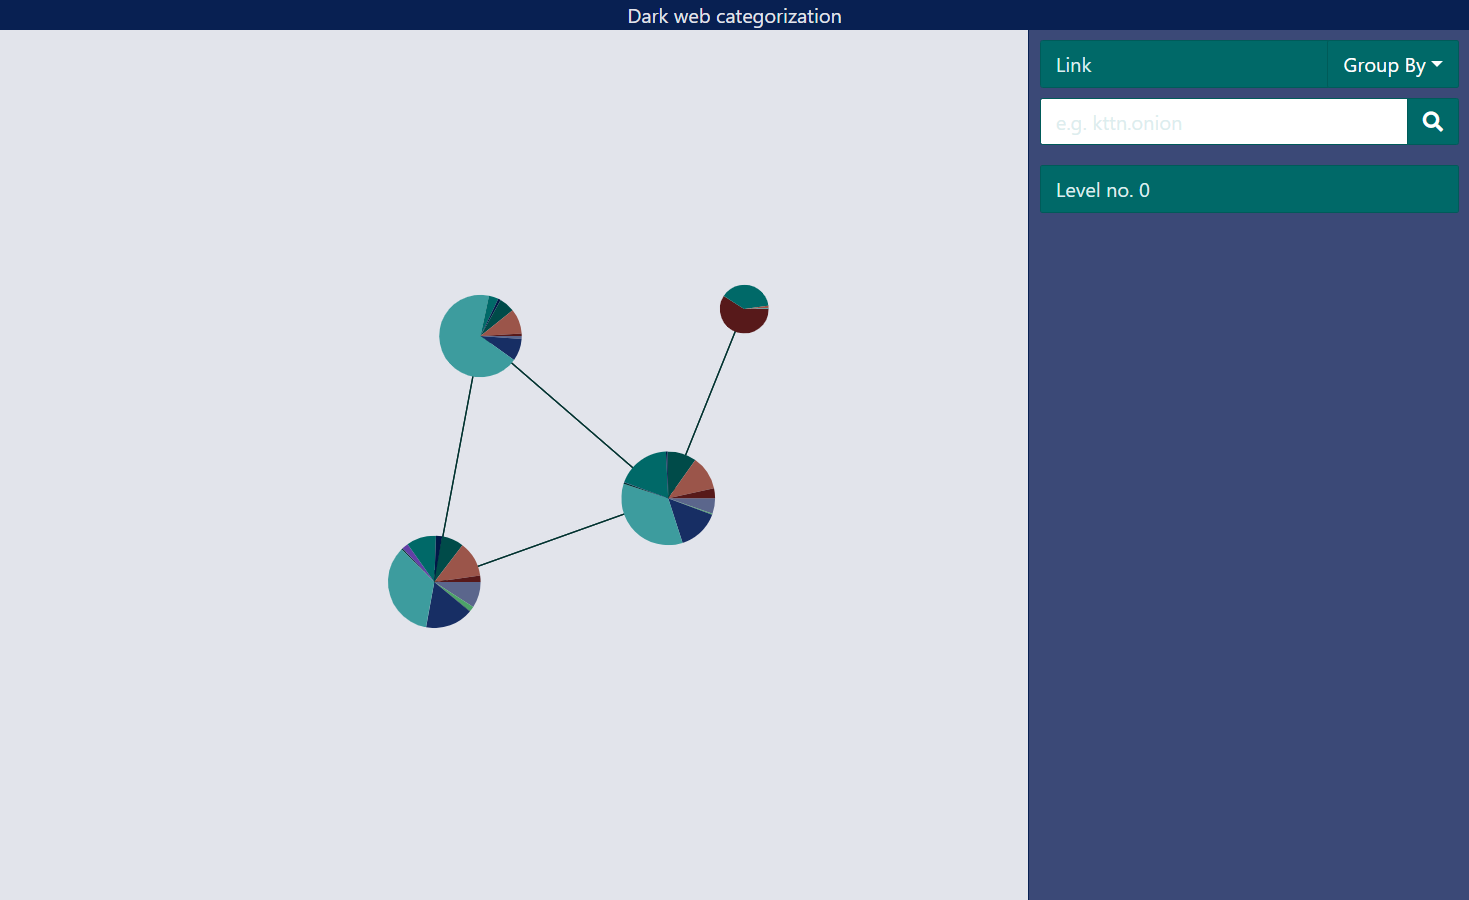
\includegraphics[width=\textwidth]{Images/basic_view.png}
  \caption{The application UI. The red arrows and text are explanatory and not part of the UI.}
  \label{MixedGraphBasic}
\end{figure}  
We designed the UI in the following way.

The UI is composed of a \textit{header} with the name of the application \textit{Dark web categorization}, a \textit{graph} and a \textit{sidebar} as can be observed in Figure \ref{MixedGraphBasic}. 

The graph-nodes represent either the communities pages are partitioned into, or the pages themselves. Both are exampled in Figure \ref{MixedGraphBasic}. The explanation of the visual differences follows.
\begin{description}
    \item[Community]  nodes are depicted as \textit{pie charts}. The individual sectors of the \textit{pie chart} represent the category makeup of the community members\footnote{Pages belonging into the community.}. We call these communities decomposable. Otherwise it is portrayed as a community-node. 
    \item[Page] nodes are portrayed as square shaped symbols. The colour of the square corresponds to the category of the page.
\end{description}  

Community-nodes can be double-clicked. After doing so, a new graph is shown. The data of this graph consist of the sub-communities of the clicked community. We call this process \textit{zooming}. If further zooming is not possible, the user reached the maximum zooming level. Each community may have a different maximum level, depending on the number of its pages and its structure. If a community at the maximum level has no siblings it is displayed in one of two ways. The community is decomposed into page-nodes if it contains at most 30 members.

If the graph contains any isolated nodes a mock-community is displayed containing all isolates. This community cannot be zoomed into. 

A button with a question mark is positioned in the upper left corner of the UI. If clicked, a legend with the available categories and their colours is shown. The legend is labeled \textit{colour legend} in Figure \ref{MixedGraphBasic}.

Arrows between nodes symbolize the links between pages or communities as is illustrated in Figure \ref{MixedGraphBasic}. Each link has a label in the form of \textit{>x/y>} assigned to it. Where \textit{x} is the number of links of the source node with a common destination. And \textit{y} is the total number of outgoing links from the source node. The direction is implied by the \textit{>} symbols. For instance, the exampled link in Figure \ref{MixedGraphBasic} indicates the lila page linking to the community with one out of a total of one links. Bidirectional links have two indicators assigned.

At the very top of the \textit{sidebar} a \textit{drop-down button} (DD) is present. It is labeled as \textit{group mode} in Figure \ref{MixedGraphBasic}. The DD configures the mode according to which the pages are grouped into. There are two modes available, \textit{link-mode} and \textit{category-mode}. If \textit{link-mode} is selected, the pages are divided into communities. If \textit{category-mode} is selected, the pages are divided into groups by categories. Zooming into such a group results in its pages being further divided into communities as if in \textit{link-mode}. 

Underneath, a filter consisting of an \textit{input field} with a \textit{submit button} was placed. The filter is also visible in Figure \ref{MixedGraphBasic}. The purpose of this element is the filtering of nodes according to a search phrase.

A level indicator is placed below the filter. The indicator marks the current level - how many times the user zoomed into a community. It is labeled as \textit{zoom level} in Figure \ref{MixedGraphBasic}. The indicator has a \textit{zoom-out button} placed next to it. After this button is clicked, the user is shown the communities of the previous level.

After single-clicking a node additional information is exampled in the \textit{sidebar}. The details vary depending on whether the node is representing a community or a single page.
The details of an individual page are as follows: 
\begin {description}
	\item [Url] which also serves as a unique identificator of the page. 
	\item [Category] of the page. Each page belongs to exactly one category.
	\item[Linked pages] are url addresses to other pages. There are up to 30 links visible in the sidebar. 
\end{description}

The details of a community are visible in Figure \ref{MixedGraphBasic}. They consist of grouped information of its members and include the following:
\begin {description}
	\item[Number of members] represents the number of all the pages belonging into the community. 
	\item [Number of domains] is the quantity of domains in the community.
	\item [First urls] addresses of members belonging into the community. There are up to 30 urls visible in the sidebar. 
	\item [Categories] are the category makeup of the members. Each category is represented by its name and the number of members belonging into this category.
\end{description}

A link for the acquisition of further node information is present in the \textit{sidebar}. The link is labeled as \textit{details link} in Figure \ref{MixedGraphBasic}. If clicked, a pop-up window with detail-options is displayed. Details may include the \textit{title}, \textit{category}, page \textit{content} and \textit{links}, depending on the user's selection. \textit{Urls} of the page or pages are present by default. The pop-up window can be observed in Figure \ref{detailsOptionsPopup}. After selecting the options and clicking the \textit{download button}, a \textit{JSON file} with the desired information is downloaded.
\begin{figure}[ht!]
  \centering
  
\includegraphics[width=0.9\textwidth]{Images/options_popup.png}
  \caption{The pop-up window with detail-options for selection. These options dictate which details will be included in the downloaded text file.}
  \label{detailsOptionsPopup}
\end{figure} 

\subsection{Technology overview}
\textit{JavaScript} \cite{javaScript} (JS) is the most favoured programming language used for creating web applications \cite{jsGithut}. It is an interpreted language supported by all modern browsers. It is open-source and as such disposes of a considerable community with convenient documentation. \textit{JS} is not strongly typed and the code might therefore be complicated to read or navigate. For this reason the FE was written in \textit{TypeScript} (TS) \cite{typeScript} which is a superset of \textit{JS} with the advantage of being typed. There is a significant number of tools and libraries for implementing UI in a clean and timely manner created for both \textit{JS} and \textit{TS}. One of such tools is the framework \textit{React.js} \cite{react} (React). \textit{React} is one of the most favoured \textit{JS} frameworks \cite{reactPopularity}. The advantages of using \textit{React} are readable code and improved performance by managing the re-rendering of page elements.

To achieve a satisfying user experience the app needed to be interactive and obtain new or modified data frequently. Repeated requests to the BE would mean longer wait time for the user. A proper mechanism for data-storing would present a convenient solution to this issue and make the requests unnecessary. A \textit{JS} library which handles the app state and works well with \textit{TS} and \textit{React} is called \textit{Redux.js} \cite{redux} (Redux). \textit{Redux} is a single store approach. This ensures easy hydration\footnote{The process of filling the attributes of an object with values.}. \textit{Redux} also provides a custom set of \textit{TS} typings and provides the developers with easy to use debugging tools. Another advantage of this library is the documentation.

The visual aspect is implemented using Less \cite{less} which is a language extending \textit{CSS} with improvements such as the possibility of using variables.

The visualization of the web graph alone was realized using the \textit{react-d3-graph} library \cite{reactD3Graph} (RD3). \textit{RD3} is 
an implementation of the library \textit{D3.js} \cite{d3} made more convenient for the use with \textit{React}. 

\subsection{Implementation} \label{FEImplementation}
The FE project consists of three main directories, unit tests, and several configuration files. This subsection describes the most important directories in the \texttt{src} directory. 
\begin{description}
    \item[\texttt{\_customized\_react-d3-graph}] contains the customized react-d3-graph module \cite{reactD3Graph} written by Daniel Caldas. A portion of the modifications were written by Antonin Klopp-Tosser in an open pull-request \cite{reactD3GraphPR}. 

We enhanced the module so that arrow-heads pointing to custom shaped nodes are visible. This was achieved by determining the direction vector of the link, normalizing it and then multiplying the vector by the shortest distance between the borders of the source and the target node.
    \item[\texttt{models}] contains models and their interfaces. Each file contains one server-model and one client-model. The conversion between these models is conducted in specific helper functions. The advantage of this approach is the independence of client-models from the BE models.
    \item[\texttt{styles}] holds the \textit{Less} classes. The classes are divided into files according to the element they are meant to modify.
    \item[\texttt{utils}] folders enclose helper functions such as converters between server and client models.
    \item[\texttt{constants}] folders hold string constants or simple functions which return a string depending on the input. 
    \item[\texttt{components}] folders contain files with \textit{React} components. Components define the skeleton of the UI with the specified behaviour.
    \item[\texttt{containers}] folders hold files with \textit{React} containers. A container is a file with access to the app-state. It is responsible for passing data to components. 
    \item[\texttt{@types}] encompasses custom typings for libraries which do not provide own typings. Typings for popular libraries are often downloadable as modules.
\end{description}
The remaining directories represent some part of the app-state management by the \textit{Redux} framework. We enclose the structure of the remaining folders in Appendix \ref{dixModifyReduxState} as it complies to the standard \textit{Redux} file structure.
